\documentclass[18pt,a4paper]{article}

%preamble



\usepackage{graphicx}
\usepackage[utf8]{inputenc}
\usepackage{amsmath}
\usepackage{enumitem}
\usepackage{multirow}
\usepackage{caption}
\usepackage{authblk}

\author[1,*]{Md Shamsuzzoha Bayzid}
\author[1,2]{Mahjabin Nahar}
\author[1,2]{Md Shariful Islam Bhuyan}
\author[1,2]{Md Saidur Rahman}
\affil[1]{Department of Computer Science and EngineeringBangladesh University of Engineering and Technology}
\affil[*]{Corresponding author: shams bayzid@cse.buet.ac.bd}
\affil[2]{yThese authors contributed equally to this work}

\title{CSE 300: Online Assignment}
\date{\today}

\usepackage{siunitx} % Required for alignment
\sisetup{
  round-mode          = places, % Rounds numbers
  round-precision     = 2, % to 2 places
}

\begin{document}
\maketitle
%\pagenumbering{arabic}
\section{Introduction}
This assignment has been designed to assess the preparation of the students in writing
scientific articles using \LaTeX. Different components,
 that are frequently used in scientific
manuscripts, have been covered in this assignment.


\subsection{Tables}
We wish to place Table 1 right here.

\begin{table}[h!]
	\label{tab1}
	\caption{\textbf{Optimization scores for Method-1 
	and Method-2 on different datasets covering 
	 various  model  conditions.}
	  We  show  average  scores  of  two  optimization 
	  criteria for various model conditions.}
	\begin{tabular}[h]{| l | c r | r r | r c |}
		\hline
		\multicolumn{3}{|c|}{Simulation Condition}
		&
		\multicolumn{4}{c|}{Optimization Score} \\
		\hline
		\multirow{2}{*}{Dataset}
		&
		\multirow{2}{*}{Complexity}
		&
		Model
		&
		\multicolumn{2}{c|}{Score 1}
		& 
		\multicolumn{2}{c |}{Score 2}
		\\
		\cline{4-7}
		&
		&
		condition
		&
		Method-1
		&
		Method-2
		&
		Method-1
		&
		Method-2
		\\
		\hline
		\hline
		
		\multirow{4}{*}{D1}
		&
		\multirow{2}{*}{Easy}
		&
		$M_1$
		&
		7,425.55
		& 770.00
		& 
		929.55
		& 10
		\\
		&
		&
		
		$M_2$
		&
		7,657.00
		& 9,179.00
		& 
		716.15
		& 20
		\\
		\cline{2-7}

		&
		\multirow{2}{*}{Hard}
		&
		$M_3$
		&
		54.00 
		& 9,007.15
		& 
		3,759.00 
		& 30
		\\
		&
		&
		
		$M_4$
		&
		74.00
		& 5567.15
		& 
		99.00
		& 25
		\\
		\hline
		\hline
		
		\multirow{3}{*}{D3}
		&
		\multirow{3}{*}{ Moderate}
		&
		$M_1$
		&
		34.00 
		& 273.00
		& 
		321.60
		& 34
		\\
		&
		&
		$M_2$
		&
		\multicolumn{2}{c|}{Not Applicable}
		& 321.60
		& 34
		\\
		
		&
		&
		$M_3$
		&
		657.00
		& 179.60
		&
		 321.60
		& 34
		\\
		\hline

	\end{tabular}
\end{table}

\subsection{Figures}
We intend to put Figure 1 at the top of a page

\begin{figure}
	\centering
	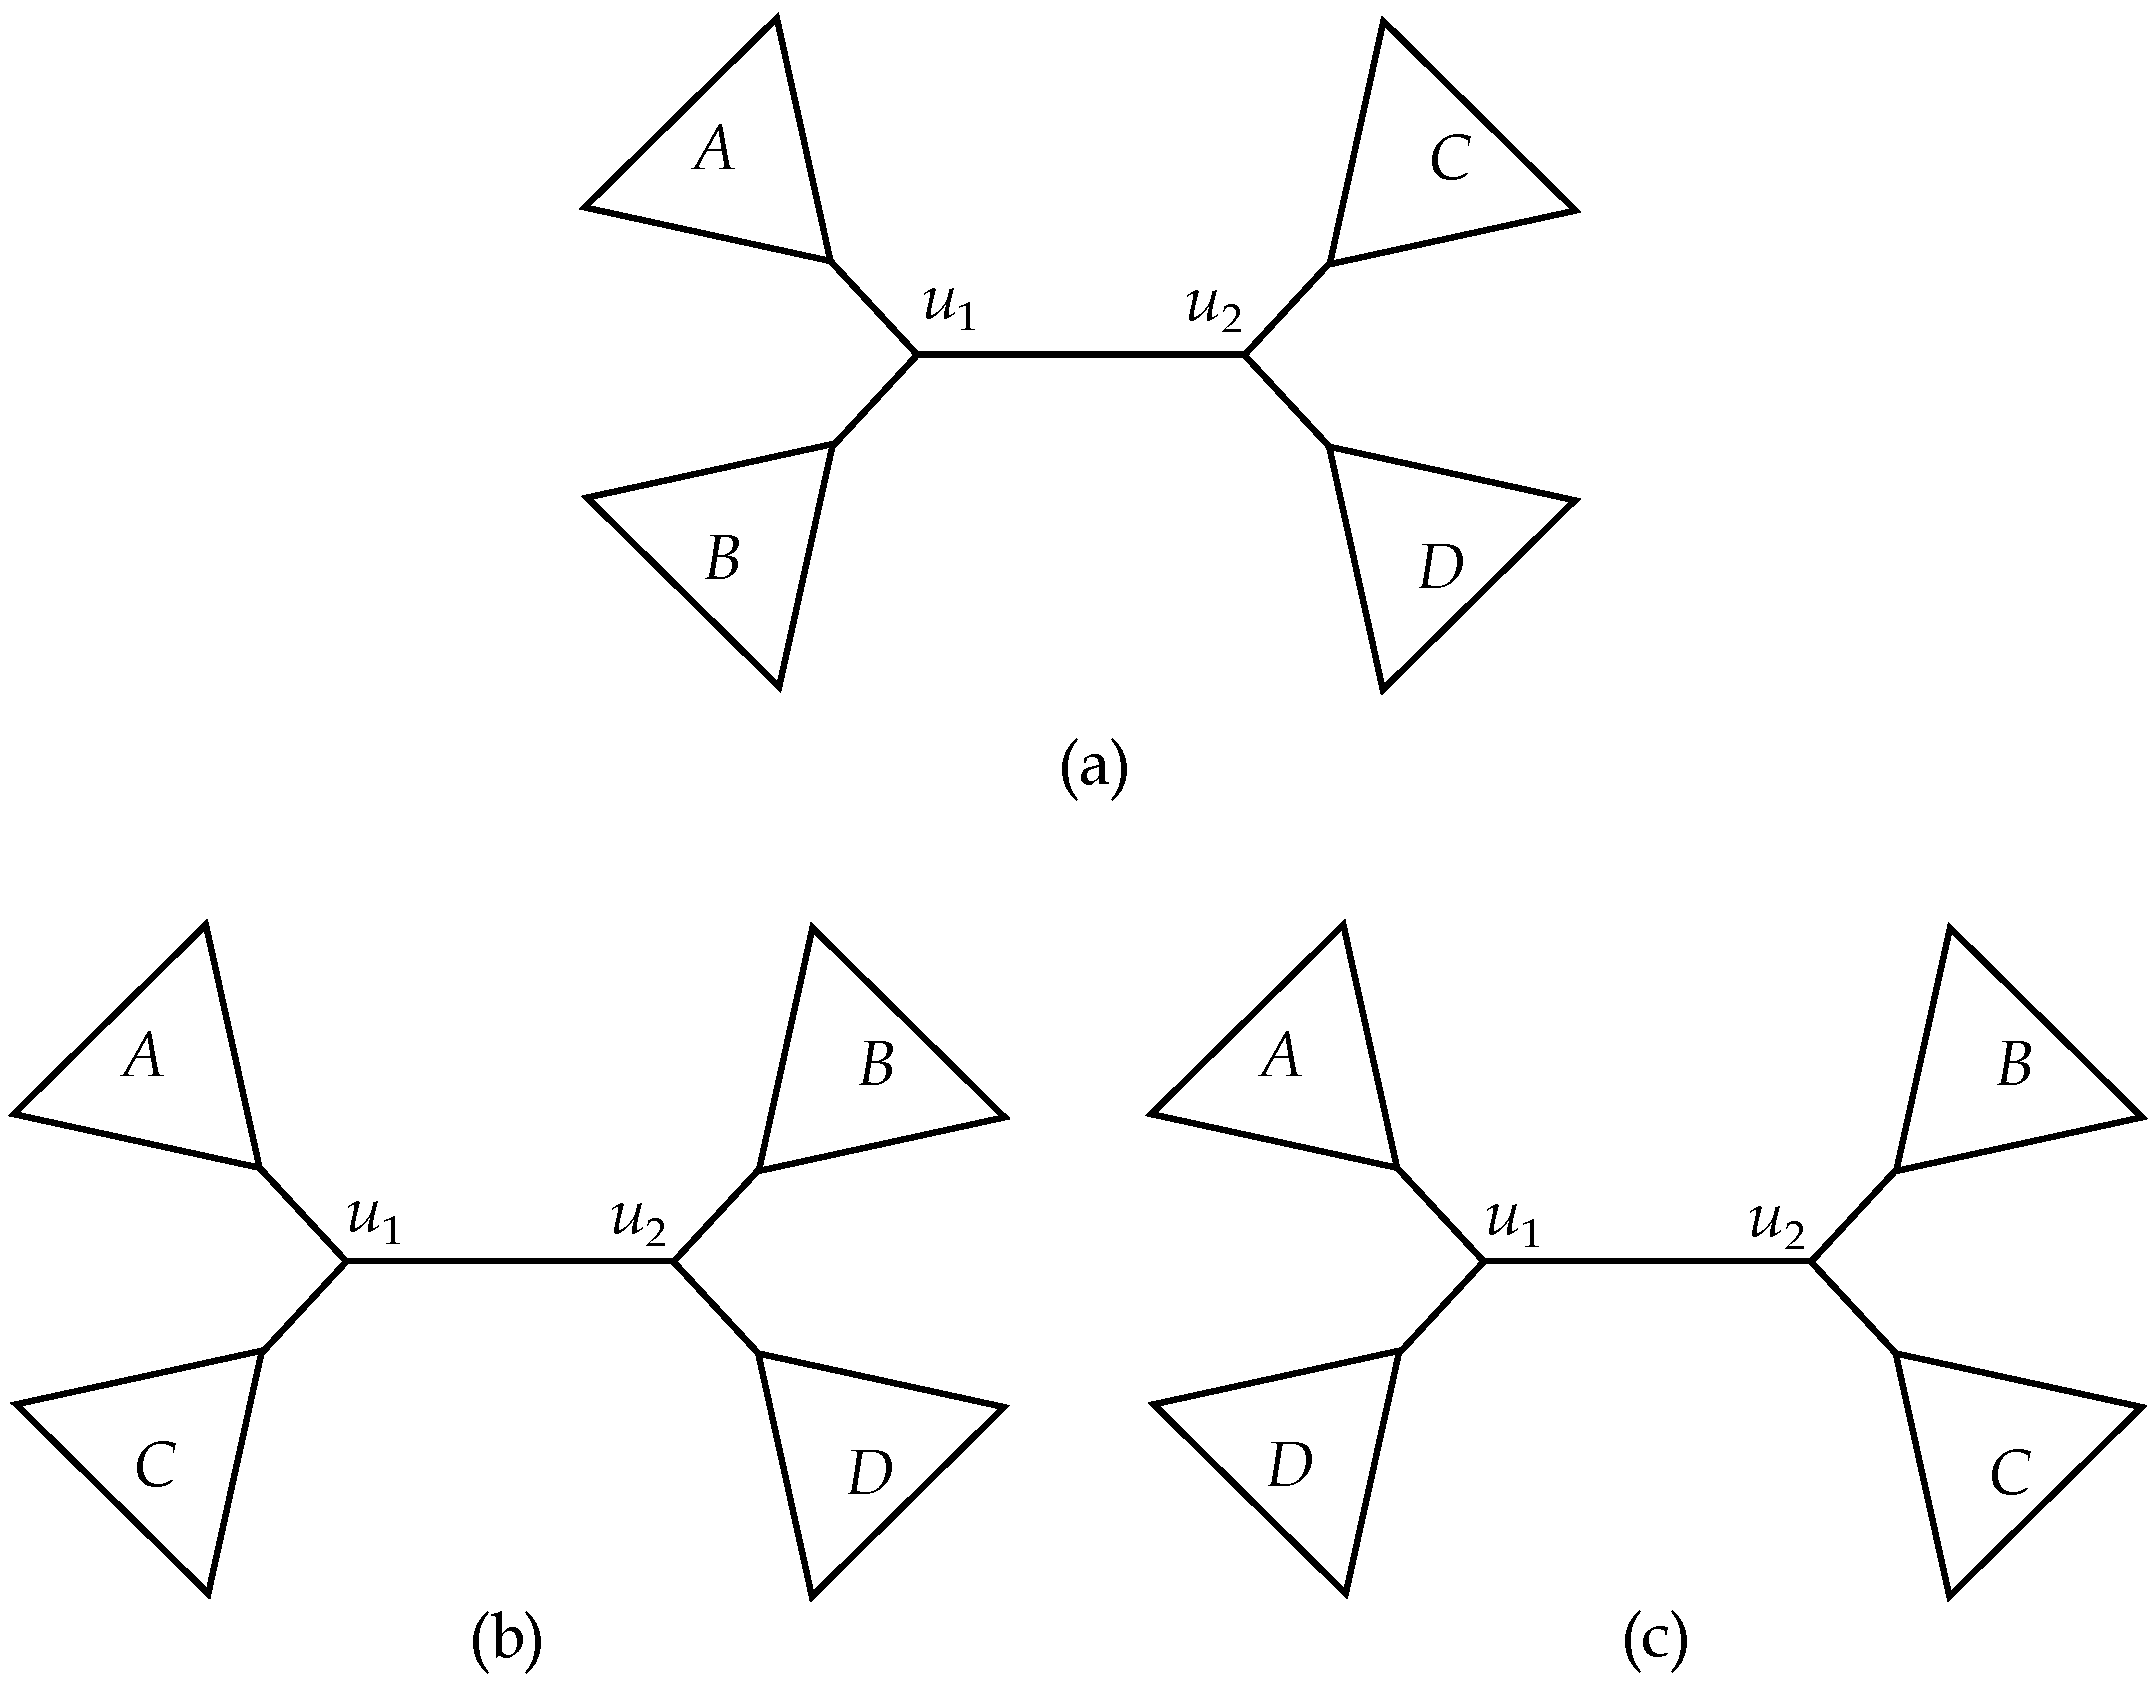
\includegraphics[scale = .3 , width = \linewidth]{Figure3.pdf}
	\caption{\textbf{Nearest Neighbor Interchange (NNI) move on an internal edge}}
\end{figure}

\subsection{ Mathematical Equations}

Let $n_1|n_2|n_3$ 
be  a  tripartition  defined  on  an  internal  node
$u$ of  a  binary  tree $T$. 
The number of tripartitions mapped to $u$ is given by Eqn. \ref{eqn}.

\begin{equation}
	\label{eqn}
	\begin{split}
	\mathcal{NQ}(n_1,n_2,n_3) & = \binom{n_1}{2} \binom{n_2}{1}
	\binom{n_3}{1} + \binom{n_2}{2} 
	\binom{n_1}{1} \binom{n_3}{1} + \binom{n_3}{2}
	\binom{n_1}{1} \binom{n_2}{1} \\
	&= \frac{n_1 n_2 n_3 ( n_1 + n_2 + n_3 -3 )}{2}
\end{split}
\end{equation}



\section{Conclusions}
The major objectives of this assignment are listed below 
(please do not ignore the fontsizes).

\begin{itemize}
\item {\huge To assess the ability of 
the students in preparing manuscriptsin \LaTeX .}
\item {\large To see if the students have 
adequately practiced different aspects ofwriting in \LaTeX.}
\item { \small To see if the students can add various basic components 
(e.g., tables, figures, equa-tions) to a \LaTeX manuscrip.}
\item {\tiny To see if the students can leverage the available materials
 (both offline and online) to dosomething which has not explicitly been taught
  in the class.}
\end{itemize}

\end{document}